% BDC223 Lecture 10: Plant Stress. Summary slides with TikZ figures.
% Curves labelled "schematic" are conceptual. Numbers on data slides come from the cited papers:
%   Davison et al. (1989) MEPS 58: 123-131; Oliver et al. (2018) Nat. Commun. 9: 1324;
%   Zhao et al. (2017) PNAS 114: 9326-9331; Wernberg et al. (2016) Science 353: 169-172 and Wernberg (2021);
%   Hammond et al. (2022) Nat. Commun. 13: 1761; Zandalinas et al. (2021) New Phytol. 230: 1034-1048.
\documentclass[aspectratio=169,11pt]{beamer}
\usepackage[sfdefault,lining]{FiraSans}
\usepackage{amsmath}
\usefonttheme{professionalfonts}
\usepackage{firamath-otf}
\setmathrm{Fira Sans}
\usepackage{tikz}
\usepackage{pgfplots}
\usepackage{array}
\pgfplotsset{compat=1.18}
\usetikzlibrary{arrows.meta,positioning,calc,shapes.geometric,decorations.pathmorphing}

\definecolor{ink}{HTML}{1F2A37}
\definecolor{accent}{HTML}{0F766E}
\definecolor{sea}{HTML}{1D4E89}
\definecolor{grey}{HTML}{6B7280}
\definecolor{leaf}{HTML}{3F8F2F}
\definecolor{warm}{HTML}{B45309}
\definecolor{hot}{HTML}{B91C1C}
\definecolor{sand}{HTML}{F2B84B}
\setbeamercolor{frametitle}{fg=white,bg=ink}
\setbeamercolor{normal text}{fg=ink,bg=white}
\setbeamercolor{itemize item}{fg=accent}
\setbeamercolor{itemize subitem}{fg=accent}
\setbeamertemplate{itemize item}{\small$\blacktriangleright$}
\setbeamertemplate{itemize subitem}{\footnotesize\textendash}
\setbeamertemplate{navigation symbols}{}
\setbeamerfont{frametitle}{size=\Large,series=\bfseries}
\setbeamertemplate{frametitle}{%
  \nointerlineskip
  \begin{beamercolorbox}[wd=\paperwidth,ht=2.4em,dp=0.9em,leftskip=1.2em]{frametitle}
    \insertframetitle
  \end{beamercolorbox}}
\setbeamertemplate{footline}{%
  \hbox to \paperwidth{\hspace{1.2em}\color{grey}\tiny BDC223 Plant Ecophysiology \textbar{} Lecture 10: Plant Stress\hfill\insertframenumber\hspace{1.2em}}\vspace{0.6em}}
\setlength{\leftmargini}{1.4em}
\hyphenpenalty=10000
\newcommand{\fignote}[1]{\par\vspace{2pt}{\color{grey}\scriptsize #1}}
\newcommand{\twocol}[2]{%
  \begin{columns}[c,onlytextwidth]
    \begin{column}{0.44\textwidth}#1\end{column}
    \begin{column}{0.54\textwidth}\centering #2\end{column}
  \end{columns}}
\tikzset{
  card/.style={draw=#1, very thick, rounded corners, fill=#1!7, align=flush left, inner sep=5pt},
  flow/.style={draw=#1, thick, rounded corners, fill=#1!8, align=center, inner sep=4pt, font=\small},
  arr/.style={-{Stealth[length=2.2mm]}, thick, grey}}

\newcommand{\pb}[1]{\begin{tikzpicture}[remember picture,overlay]
  \node[anchor=north east, font=\scriptsize\bfseries, text=white, fill=hot, rounded corners=2pt, inner sep=2pt] at ([xshift=-0.3cm,yshift=-0.1cm]current page.north east) {Planetary boundary: #1};
\end{tikzpicture}}

\begin{document}

% 1 ---------------------------------------------------------------------
\begin{frame}{What is plant stress?}
\twocol{
\begin{itemize}
  \item \textbf{Stress}: any condition that limits a plant's metabolism, growth or development
  \item \textbf{Stressor}: the external factor (heat, drought, salt, a grazer)
  \item \textbf{Strain}: the change it causes inside the plant
  \item Grime: stress is anything that limits the rate of biomass production
  \item Stress is relative: a desert is not stressful to a succulent
\end{itemize}}{
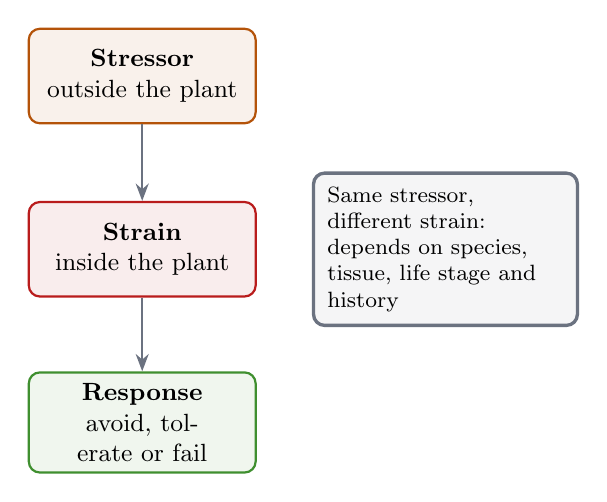
\begin{tikzpicture}[font=\small]
  \node[flow=warm, text width=2.6cm, minimum height=1.2cm] (s) at (0,2.2) {\textbf{Stressor}\\ outside the plant};
  \node[flow=hot, text width=2.6cm, minimum height=1.2cm] (t) at (0,0) {\textbf{Strain}\\ inside the plant};
  \node[flow=leaf, text width=2.6cm, minimum height=1.2cm] (r) at (0,-2.2) {\textbf{Response}\\ avoid, tolerate or fail};
  \draw[arr] (s) -- (t); \draw[arr] (t) -- (r);
  \node[card=grey, text width=3.0cm, font=\footnotesize, right=0.7cm of t] {Same stressor, different strain: depends on species, tissue, life stage and history};
\end{tikzpicture}
\fignote{After Lichtenthaler (1996) and Grime (1977).}}
\end{frame}

% 2 ---------------------------------------------------------------------
\begin{frame}{The tolerance curve}
\twocol{
\begin{itemize}
  \item Every plant performs best over a range of each factor: its \textbf{optimum}
  \item On either side: \textbf{suboptimal} zones where function declines
  \item Beyond the \textbf{tolerance limits}: damage and death
  \item Wide curve: \textbf{eurytopic} (generalist); narrow curve: \textbf{stenotopic} (specialist)
  \item Too little and too much can both be stressful
\end{itemize}}{
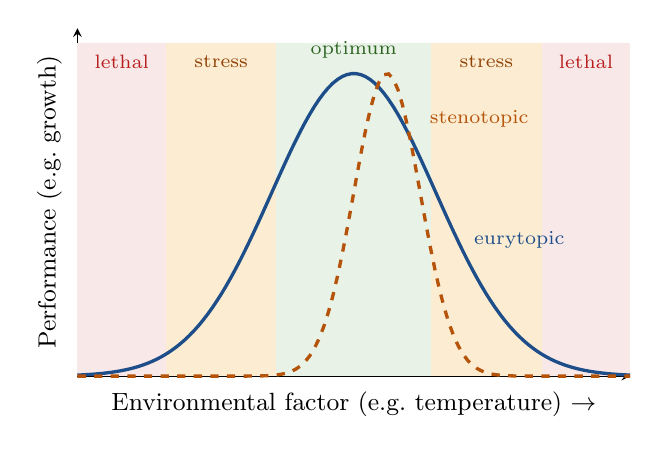
\begin{tikzpicture}
\begin{axis}[width=8.6cm, height=6.0cm, xmin=0, xmax=10, ymin=0, ymax=1.15,
  axis lines=left, xtick=\empty, ytick=\empty,
  xlabel={\small Environmental factor (e.g.\ temperature) $\rightarrow$},
  ylabel={\small Performance (e.g.\ growth)}, clip=false]
  \fill[hot!10] (axis cs:0,0) rectangle (axis cs:1.6,1.1);
  \fill[hot!10] (axis cs:8.4,0) rectangle (axis cs:10,1.1);
  \fill[sand!25] (axis cs:1.6,0) rectangle (axis cs:3.6,1.1);
  \fill[sand!25] (axis cs:6.4,0) rectangle (axis cs:8.4,1.1);
  \fill[leaf!12] (axis cs:3.6,0) rectangle (axis cs:6.4,1.1);
  \addplot[very thick, sea, domain=0:10, samples=120] {exp(-((x-5)/2.1)^2)};
  \addplot[very thick, warm, dashed, domain=0:10, samples=120] {exp(-((x-5.6)/0.85)^2)};
  \node[font=\scriptsize, leaf!70!black] at (axis cs:5,1.08) {optimum};
  \node[font=\scriptsize, warm!80!black, align=center] at (axis cs:2.6,1.04) {stress};
  \node[font=\scriptsize, warm!80!black, align=center] at (axis cs:7.4,1.04) {stress};
  \node[font=\scriptsize, hot, align=center] at (axis cs:0.8,1.04) {lethal};
  \node[font=\scriptsize, hot, align=center] at (axis cs:9.2,1.04) {lethal};
  \node[font=\scriptsize, sea, anchor=west] at (axis cs:7.0,0.45) {eurytopic};
  \node[font=\scriptsize, warm, anchor=west] at (axis cs:6.2,0.85) {stenotopic};
\end{axis}
\end{tikzpicture}
\fignote{Schematic. Zones drawn for the wide (blue) curve.}}
\end{frame}

% 3 ---------------------------------------------------------------------
\begin{frame}{Stress unfolds in time}
\begin{center}
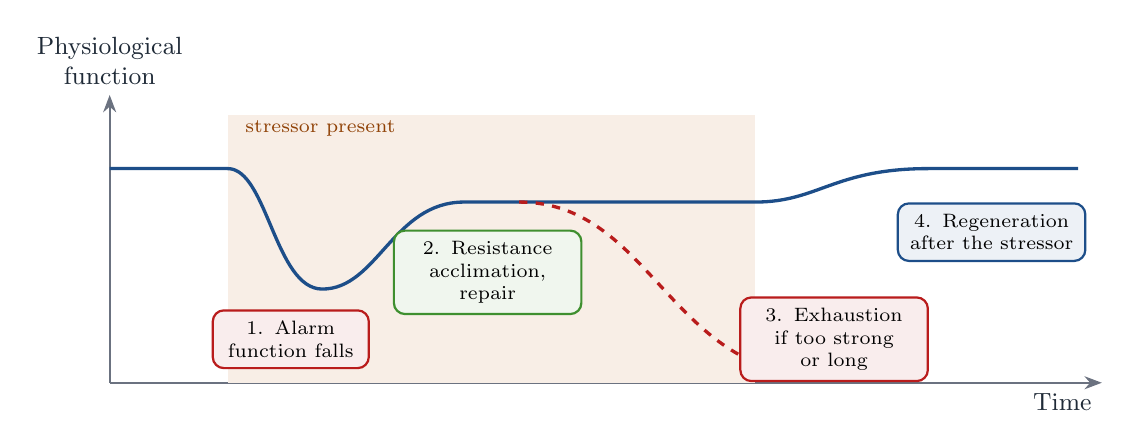
\begin{tikzpicture}[font=\small, yscale=0.85]
  \draw[arr] (0,0) -- (12.6,0) node[below left, font=\small, ink] {Time};
  \draw[arr] (0,0) -- (0,4.3) node[above, font=\small, ink, align=center] {Physiological\\function};
  \fill[warm!10] (1.5,0) rectangle (8.2,4.0);
  \node[font=\scriptsize, warm!80!black, anchor=west] at (1.6,3.8) {stressor present};
  \draw[very thick, sea] (0,3.2) -- (1.5,3.2) .. controls (2.0,3.2) and (2.1,1.4) .. (2.7,1.4)
     .. controls (3.4,1.4) and (3.6,2.7) .. (4.5,2.7) -- (8.2,2.7) .. controls (9.0,2.7) and (9.2,3.2) .. (10.4,3.2) -- (12.3,3.2);
  \draw[very thick, hot, dashed] (5.2,2.7) .. controls (6.6,2.7) and (7.0,0.9) .. (8.2,0.3) -- (8.8,0.15);
  \node[flow=hot, font=\scriptsize, text width=1.7cm] at (2.3,0.65) {1. Alarm\\ function falls};
  \node[flow=leaf, font=\scriptsize, text width=2.1cm] at (4.8,1.65) {2. Resistance\\ acclimation, repair};
  \node[flow=hot, font=\scriptsize, text width=2.1cm] at (9.2,0.65) {3. Exhaustion\\ if too strong or long};
  \node[flow=sea, font=\scriptsize, text width=2.1cm] at (11.2,2.25) {4. Regeneration\\ after the stressor};
\end{tikzpicture}
\end{center}
\fignote{Schematic, after Lichtenthaler (1996, 1998). Mild stress can harden the plant (eustress); severe stress causes lasting damage (distress).}
\end{frame}

% 4 ---------------------------------------------------------------------
\begin{frame}{The stressors}
\begin{center}
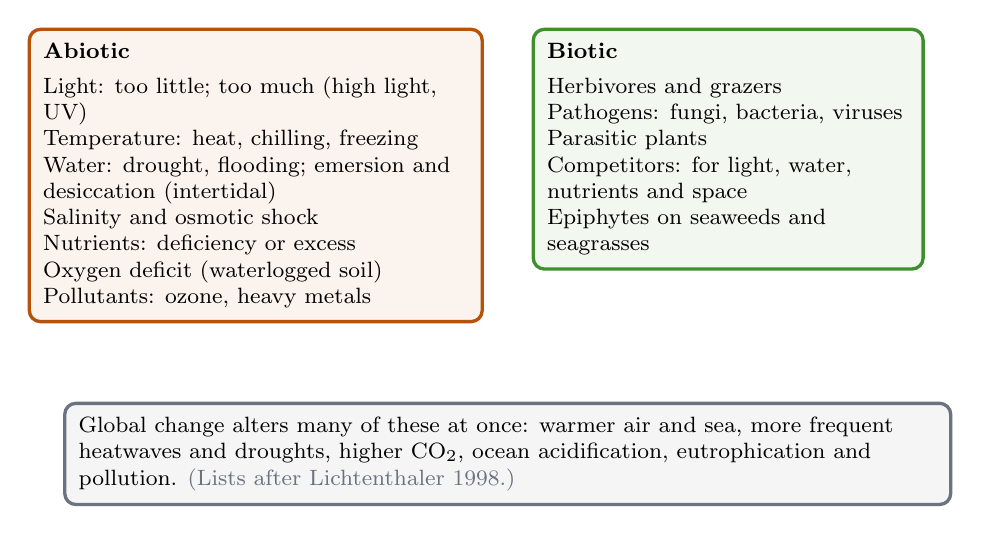
\begin{tikzpicture}[font=\small]
  \node[card=warm, text width=5.4cm, anchor=north, font=\footnotesize] (a) at (-3.0,0) {\textbf{Abiotic}\\[3pt]
    Light: too little; too much (high light, UV)\\
    Temperature: heat, chilling, freezing\\
    Water: drought, flooding; emersion and desiccation (intertidal)\\
    Salinity and osmotic shock\\
    Nutrients: deficiency or excess\\
    Oxygen deficit (waterlogged soil)\\
    Pollutants: ozone, heavy metals};
  \node[card=leaf, text width=4.6cm, anchor=north, font=\footnotesize] (b) at (3.0,0) {\textbf{Biotic}\\[3pt]
    Herbivores and grazers\\
    Pathogens: fungi, bacteria, viruses\\
    Parasitic plants\\
    Competitors: for light, water, nutrients and space\\
    Epiphytes on seaweeds and seagrasses};
  \node[card=grey, text width=10.9cm, anchor=north, font=\footnotesize] at (0.2,-4.75) {Global change alters many of these at once: warmer air and sea, more frequent heatwaves and droughts, higher CO$_2$, ocean acidification, eutrophication and pollution. {\color{grey}(Lists after Lichtenthaler 1998.)}};
\end{tikzpicture}
\end{center}
\end{frame}

% 4b --------------------------------------------------------------------
\begin{frame}{Stressors and the planetary boundaries}
\vspace{-4pt}
\centering\scriptsize
\renewcommand{\arraystretch}{1.3}
\begin{tabular}{@{}>{\raggedright\arraybackslash}p{3.3cm}>{\raggedright\arraybackslash}p{2.1cm}>{\raggedright\arraybackslash}p{8.2cm}@{}}
\textbf{Boundary (Lecture 1)} & \textbf{Status} & \textbf{Stress for plants and seaweeds}\\\hline
Climate change & \textcolor{hot}{crossed} & heat, drought, marine heatwaves, stronger winds and waves, sea-level rise\\
Ocean acidification & \textcolor{hot}{crossed (since 2025)} & coralline algae calcify less; extra CO$_2$ can favour fleshy seaweeds\\
N and P flows & \textcolor{hot}{crossed} & nutrient excess, eutrophication, epiphyte overgrowth, low oxygen\\
Freshwater change & \textcolor{hot}{crossed} & drought, flooding, salinisation; salinity change in estuaries\\
Land-system change & \textcolor{hot}{crossed} & habitat loss, fragmentation, altered microclimate\\
Biosphere integrity & \textcolor{hot}{crossed} & biotic stressors: invasive species, pathogens, altered grazing\\
Novel entities & \textcolor{hot}{crossed} & herbicides, heavy metals, plastics and other pollutants\\
Stratospheric ozone & \textcolor{leaf}{within} & UV-B stress (the ozone layer is recovering)\\
Atmospheric aerosols & \textcolor{leaf}{within} & less and more diffuse light; altered rainfall\\\hline
\end{tabular}
\fignote{Status: Richardson et al. (2023); ocean acidification from the Planetary Health Check 2025.}
\end{frame}

% 5 ---------------------------------------------------------------------
\begin{frame}{A common currency: the energy balance of photosynthesis}
\twocol{
\begin{itemize}
  \item Light capture: fast, almost insensitive to temperature
  \item CO$_2$ fixation and growth: slower; need warmth, water and nutrients
  \item Photon supply exceeds processing capacity, or sinks are impaired: excess energy builds up
  \item Sensed as \textbf{excitation pressure} on PSII
\end{itemize}}{
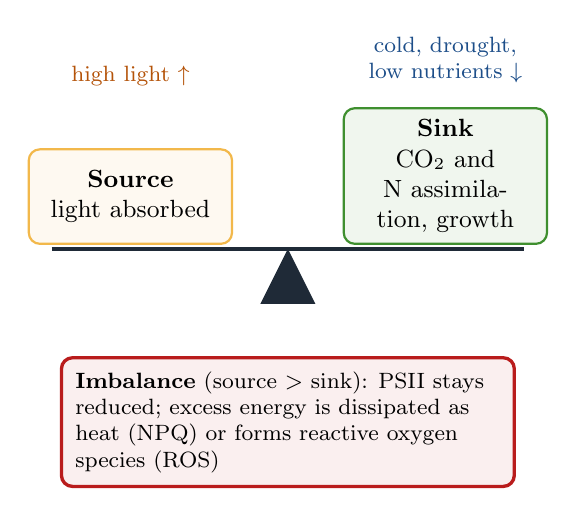
\begin{tikzpicture}[font=\small]
  \draw[very thick, ink] (-3,0) -- (3,0);
  \fill[ink] (0,0) -- (-0.35,-0.7) -- (0.35,-0.7) -- cycle;
  \node[flow=sand, text width=2.3cm, minimum height=1.2cm, anchor=south] at (-2.0,0.05) {\textbf{Source}\\ light absorbed};
  \node[flow=leaf, text width=2.3cm, minimum height=1.2cm, anchor=south] at (2.0,0.05) {\textbf{Sink}\\ CO$_2$ and N assimilation, growth};
  \node[card=hot, text width=5.4cm, font=\footnotesize] at (0,-2.2) {\textbf{Imbalance} (source $>$ sink): PSII stays reduced; excess energy is dissipated as heat (NPQ) or forms reactive oxygen species (ROS)};
  \node[font=\footnotesize, warm, align=center] at (-2.0,2.2) {high light $\uparrow$};
  \node[font=\footnotesize, sea, align=center] at (2.0,2.4) {cold, drought,\\ low nutrients $\downarrow$};
\end{tikzpicture}
\fignote{After Huner et al. (1998).}}
\end{frame}

% 6 ---------------------------------------------------------------------
\begin{frame}{Reactive oxygen species: signal and danger}
\twocol{
\begin{itemize}
  \item ROS (singlet oxygen, superoxide, H$_2$O$_2$, hydroxyl radical) form in chloroplasts and mitochondria
  \item Almost every stress raises ROS production
  \item \textbf{Low levels}: signals that switch on acclimation
  \item \textbf{High levels}: damage to lipids, proteins and DNA
  \item Antioxidants (enzymes, ascorbate, glutathione, carotenoids) keep the balance
\end{itemize}}{
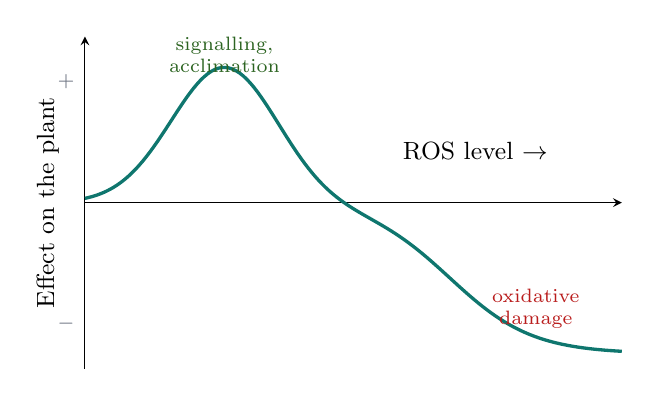
\begin{tikzpicture}
\begin{axis}[width=8.4cm, height=5.8cm, xmin=0, xmax=10, ymin=-1.1, ymax=1.1,
  axis lines=middle, xtick=\empty, ytick=\empty, clip=false,
  xlabel={\small ROS level $\rightarrow$}, x label style={at={(axis description cs:0.88,0.6)}},
  ylabel={\small Effect on the plant}, y label style={at={(axis description cs:-0.03,0.5)}, rotate=90, anchor=south}]
  \addplot[very thick, accent, domain=0:10, samples=150] {0.9*exp(-((x-2.6)/1.4)^2) - 1.0/(1+exp(-(x-6.8)*1.3))};
  \node[font=\scriptsize, leaf!70!black, align=center] at (axis cs:2.6,0.98) {signalling,\\ acclimation};
  \node[font=\scriptsize, hot, align=center] at (axis cs:8.4,-0.7) {oxidative\\ damage};
  \node[font=\scriptsize, grey] at (axis cs:-0.35,0.8) {+};
  \node[font=\scriptsize, grey] at (axis cs:-0.35,-0.8) {$-$};
\end{axis}
\end{tikzpicture}
\fignote{Schematic, after Apel and Hirt (2004) and Mittler et al. (2022).}}
\end{frame}

% 7 ---------------------------------------------------------------------
\begin{frame}{Measuring stress with chlorophyll fluorescence}
\twocol{
\begin{itemize}
  \item $F_v/F_m$: maximum quantum yield of PSII (Lecture 7b)
  \item Unstressed plants: about 0.8
  \item A fall shows that PSII is down-regulated or damaged
  \item \textbf{Full recovery} once the stressor is removed: photoprotection (dynamic)
  \item \textbf{Slow or partial recovery}: damage (chronic)
  \item Fast, non-destructive; works in the field and on the shore
\end{itemize}}{
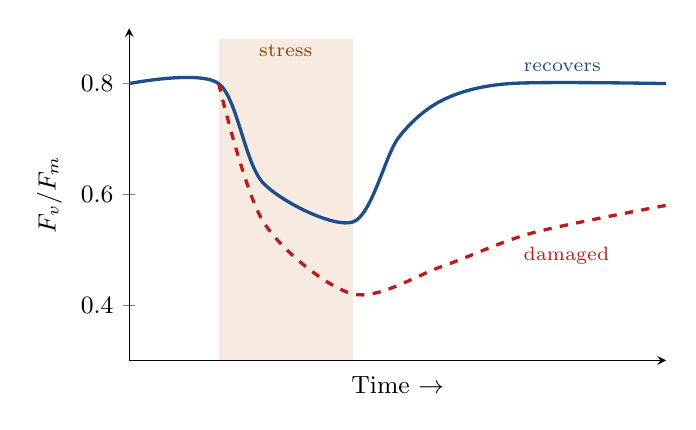
\begin{tikzpicture}
\begin{axis}[width=8.4cm, height=5.8cm, xmin=0, xmax=12, ymin=0.3, ymax=0.9,
  axis lines=left, xtick=\empty, ytick={0.4,0.6,0.8}, yticklabel style={font=\small},
  xlabel={\small Time $\rightarrow$}, ylabel={\small $F_v/F_m$}, clip=false]
  \fill[warm!12] (axis cs:2,0.3) rectangle (axis cs:5,0.88);
  \node[font=\scriptsize, warm!80!black] at (axis cs:3.5,0.86) {stress};
  \addplot[very thick, sea, smooth] coordinates {(0,0.8) (2,0.8) (3,0.62) (5,0.55) (6,0.70) (7,0.77) (8.5,0.8) (12,0.8)};
  \addplot[very thick, hot, dashed, smooth] coordinates {(2,0.8) (3,0.55) (5,0.42) (7,0.47) (9,0.53) (12,0.58)};
  \node[font=\scriptsize, sea, anchor=west] at (axis cs:8.6,0.83) {recovers};
  \node[font=\scriptsize, hot, anchor=west] at (axis cs:8.6,0.49) {damaged};
\end{axis}
\end{tikzpicture}
\fignote{Schematic. Healthy value from Maxwell and Johnson (2000).}}
\end{frame}

% 8 ---------------------------------------------------------------------
\begin{frame}{Three outcomes}
\begin{center}
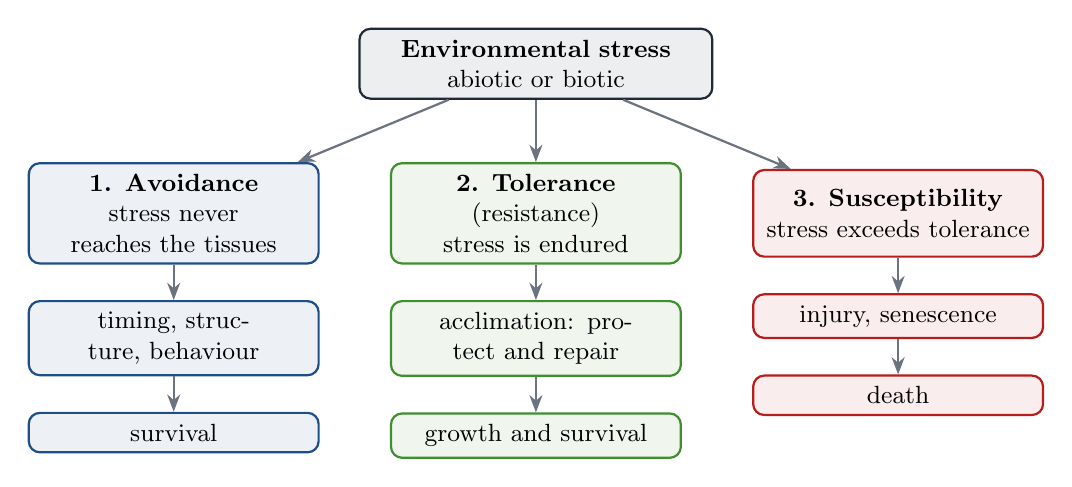
\begin{tikzpicture}[font=\small, node distance=0.45cm]
  \node[flow=ink, text width=4.2cm] (st) at (0,0) {\textbf{Environmental stress}\\ abiotic or biotic};
  \node[flow=sea, text width=3.4cm, minimum height=1.1cm] (av) at (-4.6,-1.9) {\textbf{1. Avoidance}\\ stress never reaches the tissues};
  \node[flow=leaf, text width=3.4cm, minimum height=1.1cm] (to) at (0,-1.9) {\textbf{2. Tolerance}\\ (resistance) stress is endured};
  \node[flow=hot, text width=3.4cm, minimum height=1.1cm] (su) at (4.6,-1.9) {\textbf{3. Susceptibility}\\ stress exceeds tolerance};
  \node[flow=sea, below=of av, text width=3.4cm] (av2) {timing, structure, behaviour};
  \node[flow=leaf, below=of to, text width=3.4cm] (to2) {acclimation: protect and repair};
  \node[flow=hot, below=of su, text width=3.4cm] (su2) {injury, senescence};
  \node[flow=sea, below=of av2, text width=3.4cm] (av3) {survival};
  \node[flow=leaf, below=of to2, text width=3.4cm] (to3) {growth and survival};
  \node[flow=hot, below=of su2, text width=3.4cm] (su3) {death};
  \foreach \a/\b in {st/av,st/to,st/su,av/av2,av2/av3,to/to2,to2/to3,su/su2,su2/su3} \draw[arr] (\a) -- (\b);
\end{tikzpicture}
\end{center}
\end{frame}

% 9 ---------------------------------------------------------------------
\begin{frame}{Avoidance in time}
\twocol{
\begin{itemize}
  \item \textbf{Ephemerals}: live only in the favourable season; seeds survive the rest
  \item \textbf{Deciduous} plants drop leaves before winter or drought
  \item \textbf{Dormancy}: buds, bulbs, seeds, spores
  \item \textbf{Heteromorphic} seaweeds: upright blades alternate with a crust or microscopic stage that resists grazing
\end{itemize}}{
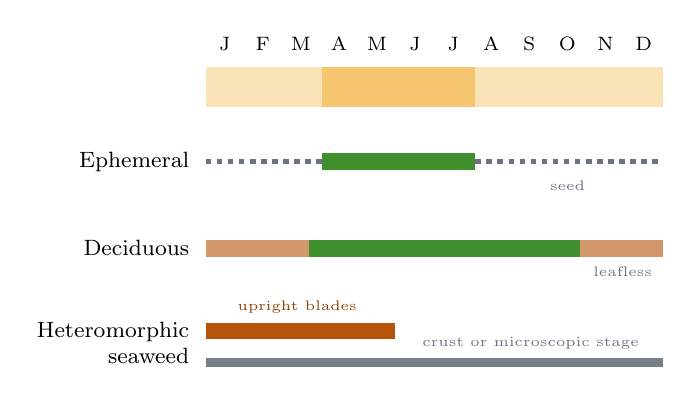
\begin{tikzpicture}[font=\scriptsize]
  \begin{scope}[xscale=0.78]
  \foreach \m/\l [count=\i] in {J/,F/,M/,A/,M/,J/,J/,A/,S/,O/,N/,D/} \node at (\i*0.62,4.4) {\m};
  \fill[sand!40] (0.31,3.6) rectangle (7.75,4.1);   \fill[sand!80] (2.2,3.6) rectangle (4.7,4.1);
  \node[anchor=east, font=\footnotesize] at (0.2,2.9) {Ephemeral};
  \draw[line width=6pt, leaf] (2.2,2.9) -- (4.7,2.9); \draw[line width=2pt, grey, dotted] (0.31,2.9) -- (2.2,2.9) (4.7,2.9) -- (7.75,2.9);
  \node[font=\tiny, grey] at (6.2,2.6) {seed};
  \node[anchor=east, font=\footnotesize] at (0.2,1.8) {Deciduous};
  \draw[line width=6pt, leaf] (2.0,1.8) -- (6.4,1.8); \draw[line width=6pt, warm!60] (0.31,1.8) -- (2.0,1.8) (6.4,1.8) -- (7.75,1.8);
  \node[font=\tiny, grey] at (7.1,1.5) {leafless};
  \node[anchor=east, font=\footnotesize, align=right] at (0.2,0.6) {Heteromorphic\\ seaweed};
  \draw[line width=6pt, warm] (0.31,0.75) -- (3.4,0.75); \node[font=\tiny, warm!80!black] at (1.8,1.05) {upright blades};
  \draw[line width=3pt, ink!60] (0.31,0.35) -- (7.75,0.35); \node[font=\tiny, grey] at (5.6,0.6) {crust or microscopic stage};
  \end{scope}
\end{tikzpicture}
\fignote{Schematic; darker band: favourable season. Seaweed example after Lubchenco and Cubit (1980).}}
\end{frame}

% 10 --------------------------------------------------------------------
\begin{frame}{Avoidance by structure and physiology}
\begin{center}
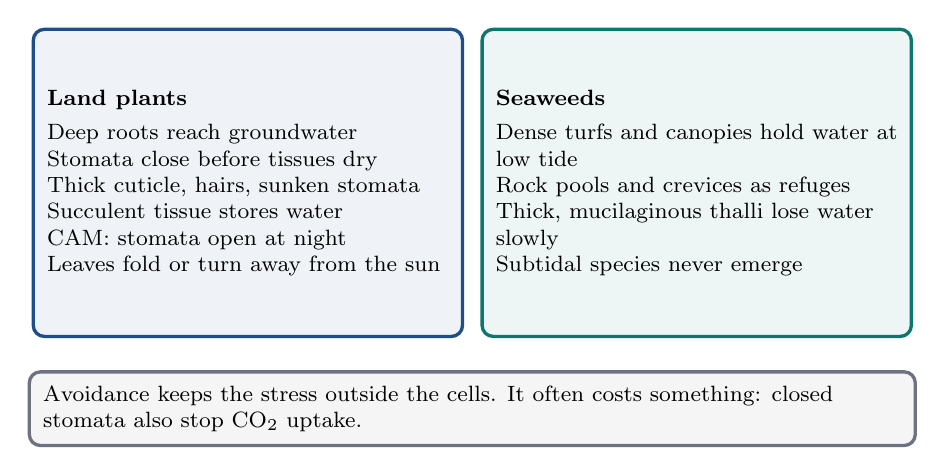
\begin{tikzpicture}[font=\small]
  \node[card=sea, text width=5.1cm, minimum height=3.9cm, anchor=north, font=\footnotesize] at (-2.85,0) {\textbf{Land plants}\\[3pt]
    Deep roots reach groundwater\\
    Stomata close before tissues dry\\
    Thick cuticle, hairs, sunken stomata\\
    Succulent tissue stores water\\
    CAM: stomata open at night\\
    Leaves fold or turn away from the sun};
  \node[card=accent, text width=5.1cm, minimum height=3.9cm, anchor=north, font=\footnotesize] at (2.85,0) {\textbf{Seaweeds}\\[3pt]
    Dense turfs and canopies hold water at low tide\\
    Rock pools and crevices as refuges\\
    Thick, mucilaginous thalli lose water slowly\\
    Subtidal species never emerge};
  \node[card=grey, text width=10.9cm, font=\footnotesize, anchor=north] at (0,-4.35) {Avoidance keeps the stress outside the cells. It often costs something: closed stomata also stop CO$_2$ uptake.};
\end{tikzpicture}
\end{center}
\end{frame}

% 11 --------------------------------------------------------------------
\begin{frame}{Tolerance: the cellular toolkit}
\begin{center}
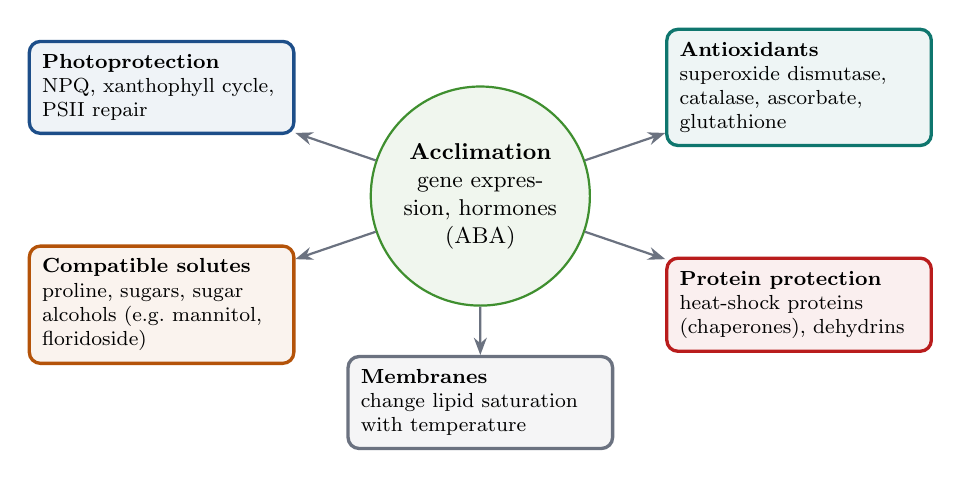
\begin{tikzpicture}[font=\small, scale=0.92, transform shape]
  \node[flow=leaf, circle, text width=2.2cm, minimum size=2.6cm] (c) at (0,0) {\textbf{Acclimation}\\ gene expression, hormones (ABA)};
  \node[card=sea, text width=3.3cm, font=\footnotesize] (a) at (-4.4,1.5) {\textbf{Photoprotection}\\ NPQ, xanthophyll cycle, PSII repair};
  \node[card=accent, text width=3.3cm, font=\footnotesize] (b) at (4.4,1.5) {\textbf{Antioxidants}\\ superoxide dismutase, catalase, ascorbate, glutathione};
  \node[card=warm, text width=3.3cm, font=\footnotesize] (d) at (-4.4,-1.5) {\textbf{Compatible solutes}\\ proline, sugars, sugar alcohols (e.g.\ mannitol, floridoside)};
  \node[card=hot, text width=3.3cm, font=\footnotesize] (e) at (4.4,-1.5) {\textbf{Protein protection}\\ heat-shock proteins (chaperones), dehydrins};
  \node[card=grey, text width=3.3cm, font=\footnotesize] (f) at (0,-2.85) {\textbf{Membranes}\\ change lipid saturation with temperature};
  \foreach \n in {a,b,d,e,f} \draw[arr] (c) -- (\n);
\end{tikzpicture}
\end{center}
\fignote{These mechanisms are switched on by the stress and switched off when it passes.}
\end{frame}

% 12 --------------------------------------------------------------------
\begin{frame}{Responses on four timescales}
\begin{center}
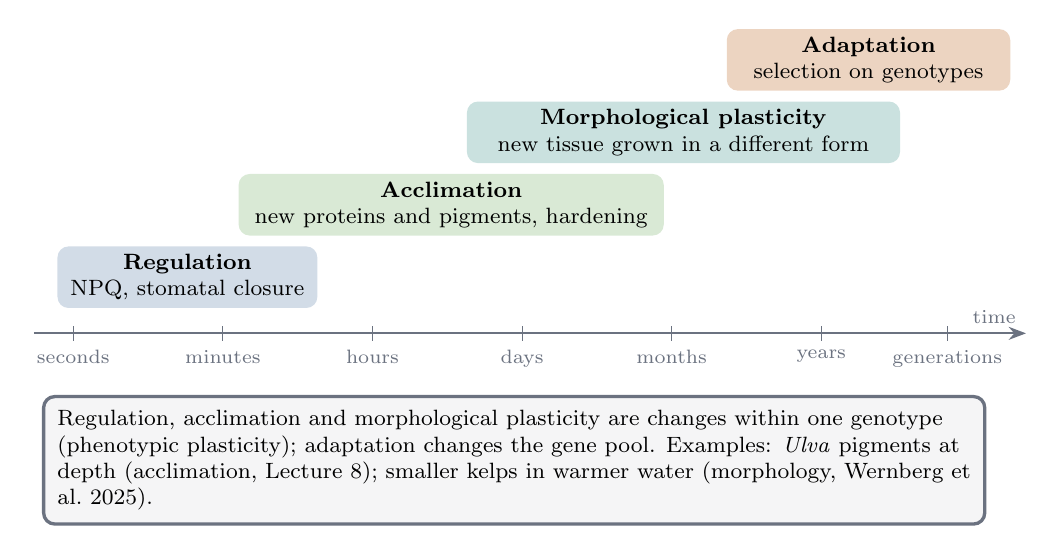
\begin{tikzpicture}[font=\small, yscale=0.92]
  \draw[arr] (0,0) -- (12.6,0) node[above left, font=\scriptsize, grey] {time};
  \foreach \x/\l in {0.5/seconds, 2.4/minutes, 4.3/hours, 6.2/days, 8.1/months, 10.0/years, 11.6/generations} {\draw[grey] (\x,0.1) -- (\x,-0.1); \node[below, font=\scriptsize, grey] at (\x,-0.1) {\l};}
  \fill[sea!20, rounded corners] (0.3,0.35) rectangle (3.6,1.2);
  \node[align=center, font=\footnotesize] at (1.95,0.775) {\textbf{Regulation}\\ NPQ, stomatal closure};
  \fill[leaf!20, rounded corners] (2.6,1.35) rectangle (8.0,2.2);
  \node[align=center, font=\footnotesize] at (5.3,1.775) {\textbf{Acclimation}\\ new proteins and pigments, hardening};
  \fill[accent!22, rounded corners] (5.5,2.35) rectangle (11.0,3.2);
  \node[align=center, font=\footnotesize] at (8.25,2.775) {\textbf{Morphological plasticity}\\ new tissue grown in a different form};
  \fill[warm!25, rounded corners] (8.8,3.35) rectangle (12.4,4.2);
  \node[align=center, font=\footnotesize] at (10.6,3.775) {\textbf{Adaptation}\\ selection on genotypes};
  \node[card=grey, text width=11.6cm, font=\footnotesize, anchor=north] at (6.1,-0.85) {Regulation, acclimation and morphological plasticity are changes within one genotype (phenotypic plasticity); adaptation changes the gene pool. Examples: \textit{Ulva} pigments at depth (acclimation, Lecture 8); smaller kelps in warmer water (morphology, Wernberg et al.\ 2025).};
\end{tikzpicture}
\end{center}
\end{frame}

% 13 --------------------------------------------------------------------
\begin{frame}{Case study: stress and zonation on the shore}
\pb{climate change}
\twocol{
\begin{itemize}
  \item Emersion: desiccation, heat or frost, high light, salinity change
  \item \textbf{Tolerance} matches shore height
  \item 3 h at $-20$\,\textdegree C: upper-shore \textit{F.\ spiralis} unaffected; low-shore \textit{F.\ edentatus} lost 97\% of photosynthesis
  \item Upper limits: physical stress; lower limits: competition, grazing
\end{itemize}}{
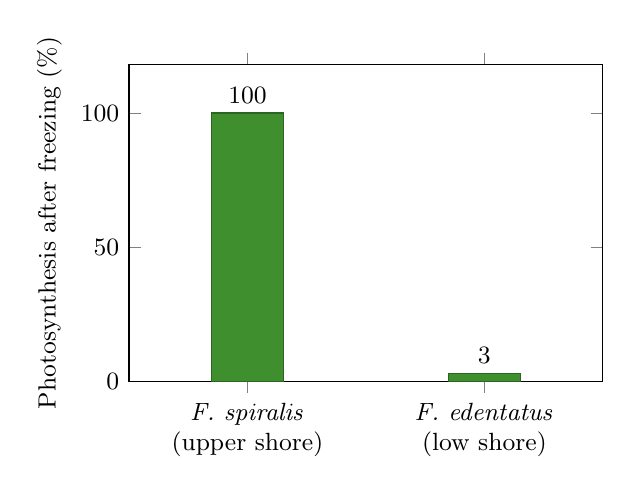
\begin{tikzpicture}
\begin{axis}[ybar, width=7.6cm, height=5.6cm, bar width=26pt, ymin=0, ymax=118,
  symbolic x coords={upper,low}, xtick=data,
  xticklabels={\textit{F. spiralis}\\(upper shore), \textit{F. edentatus}\\(low shore)},
  xticklabel style={font=\small, align=center}, yticklabel style={font=\small},
  ylabel={\small Photosynthesis after freezing (\%)},
  nodes near coords, every node near coord/.append style={font=\small}, enlarge x limits=0.5]
\addplot[fill=leaf, draw=leaf!70!black] coordinates {(upper,100) (low,3)};
\end{axis}
\end{tikzpicture}
\fignote{Davison et al. (1989); ``unaffected'' plotted as 100\%.}}
\end{frame}

% 14 --------------------------------------------------------------------
\begin{frame}{Case study: a marine heatwave and a kelp forest}
\pb{climate change, biosphere integrity}
\twocol{
\begin{itemize}
  \item Western Australia, 2011: $>$2000 km of coast, $>$10 weeks
  \item Above the net-growth limit of \textit{Ecklonia radiata} (about 23\,\textdegree C)
  \item About 43\% of west-coast kelp died; range contracted by 100 km
  \item Turfs and warm-water fishes took over; no recovery
\end{itemize}}{
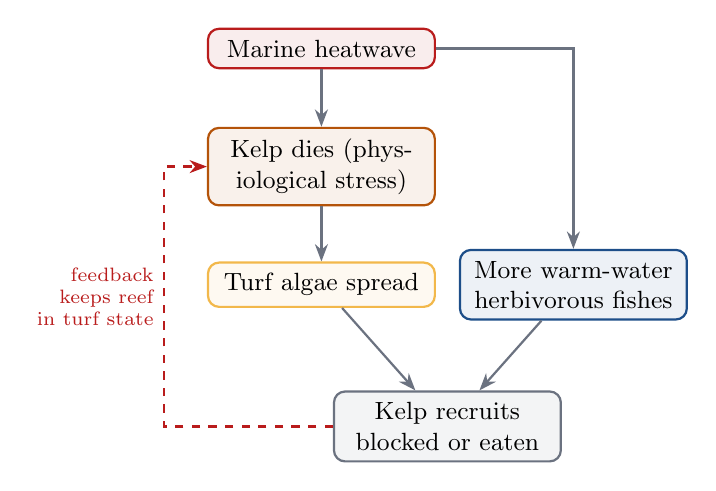
\begin{tikzpicture}[font=\small]
  \node[flow=hot, text width=2.6cm] (h) at (0,2.6) {Marine heatwave};
  \node[flow=warm, text width=2.6cm] (k) at (0,1.1) {Kelp dies (physiological stress)};
  \node[flow=sand, text width=2.6cm] (t) at (0,-0.4) {Turf algae spread};
  \node[flow=sea, text width=2.6cm] (f) at (3.2,-0.4) {More warm-water herbivorous fishes};
  \node[flow=grey, text width=2.6cm] (r) at (1.6,-2.2) {Kelp recruits blocked or eaten};
  \draw[arr] (h) -- (k); \draw[arr] (k) -- (t); \draw[arr] (h) -| (f);
  \draw[arr] (t) -- (r); \draw[arr] (f) -- (r);
  \draw[arr, hot, dashed] (r.west) -| node[pos=0.75, left, font=\scriptsize, hot, align=right] {feedback\\ keeps reef\\ in turf state} (-2.0,1.1) -- (k.west);
\end{tikzpicture}
\fignote{Wernberg et al. (2016); Wernberg (2021).}}
\end{frame}

% 15b -------------------------------------------------------------------
\begin{frame}{Case study: smaller kelps in warmer water}
\pb{climate change}
\twocol{
\begin{itemize}
  \item \textit{Laminaria pallida}, either side of the Cape Peninsula
  \item Warm False Bay site: shorter, thinner stipes, less biomass, no epiphytes
  \item Same stipe pattern in \textit{L.\ hyperborea} (Norway vs France)
  \item \textbf{Sublethal} stress: smaller kelps, less habitat
\end{itemize}}{
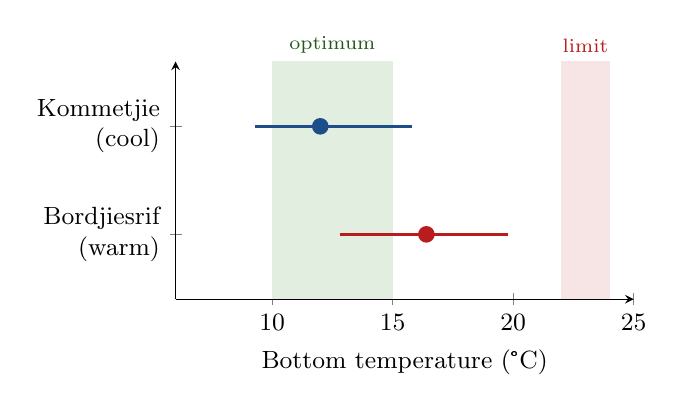
\begin{tikzpicture}
\begin{axis}[width=7.4cm, height=4.6cm, xmin=6, xmax=25, xtick={10,15,20,25}, ymin=0.4, ymax=2.6,
  ytick={1,2}, yticklabels={Bordjiesrif\\(warm), Kommetjie\\(cool)}, yticklabel style={font=\small, align=right},
  xlabel={\small Bottom temperature (\textdegree C)}, xticklabel style={font=\small}, axis lines=left, clip=false]
  \fill[leaf!15] (axis cs:10,0.4) rectangle (axis cs:15,2.6);
  \fill[hot!12] (axis cs:22,0.4) rectangle (axis cs:24,2.6);
  \node[font=\scriptsize, leaf!60!black] at (axis cs:12.5,2.75) {optimum};
  \node[font=\scriptsize, hot] at (axis cs:23,2.75) {limit};
  \draw[very thick, sea] (axis cs:9.3,2) -- (axis cs:15.8,2); \fill[sea] (axis cs:12.0,2) circle (3pt);
  \draw[very thick, hot] (axis cs:12.8,1) -- (axis cs:19.8,1); \fill[hot] (axis cs:16.4,1) circle (3pt);
\end{axis}
\end{tikzpicture}
\fignote{Mean and range of temperature; optimum and survival limit for \textit{L.\ pallida}. Wernberg et al.\ (2025).}}
\end{frame}

% 15c -------------------------------------------------------------------
\begin{frame}{Not every coast is warming}
\pb{climate change}
\twocol{
\begin{itemize}
  \item Eastern boundary upwelling systems (EBUS): stronger upwelling-favourable winds bring up more cold water
  \item Southern Benguela, 1982--2009: up to $-0.5$\,\textdegree C per decade; Agulhas Current: up to $+0.55$
  \item Eastern Agulhas Bank (summers 1983--2025): coast $-0.19$, offshore $+0.18$\,\textdegree C per decade
  \item Explore: \textbf{www.saoce.org}
\end{itemize}}{
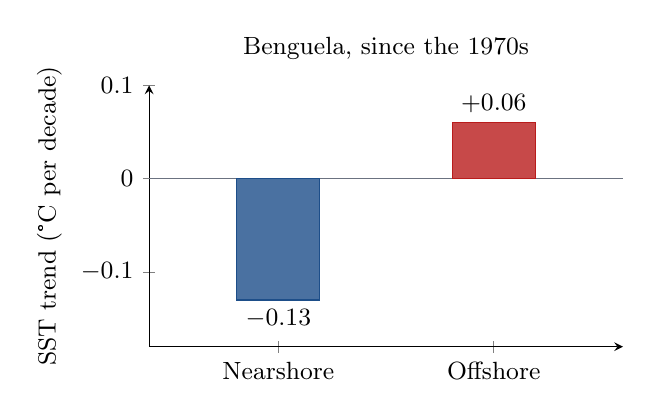
\begin{tikzpicture}
\begin{axis}[ybar, bar shift=0pt, width=7.6cm, height=4.9cm, bar width=30pt, ymin=-0.18, ymax=0.1,
  title={\small Benguela, since the 1970s}, xmin=0.4, xmax=2.6, xtick={1,2}, xticklabels={Nearshore, Offshore},
  xticklabel style={font=\small}, yticklabel style={font=\small, /pgf/number format/fixed, /pgf/number format/precision=2},
  ylabel={\small SST trend (\textdegree C per decade)}, axis x line=bottom, axis y line=left,
  nodes near coords={\pgfmathprintnumber[fixed,precision=2,showpos]{\pgfplotspointmeta}}, every node near coord/.append style={font=\small}]
\draw[grey] (axis cs:0.4,0) -- (axis cs:2.6,0);
\addplot[fill=sea!80, draw=sea] coordinates {(1,-0.13)};
\addplot[fill=hot!80, draw=hot] coordinates {(2,0.06)};
\end{axis}
\end{tikzpicture}
\fignote{Santos et al.\ (2012); Rouault et al.\ (2010); Smit et al.\ (submitted).}}
\end{frame}

% 15d -------------------------------------------------------------------
\begin{frame}{Case study: waves and swell shape kelps}
\pb{climate change}
\twocol{
\begin{itemize}
  \item West coast: open to Southern Ocean swell; False Bay: sheltered
  \item Kelp form tracked wave exposure more than temperature
  \item Temperature mattered more where waves were weak
  \item Global wave power is increasing (Reguero et al.\ 2019)
\end{itemize}}{
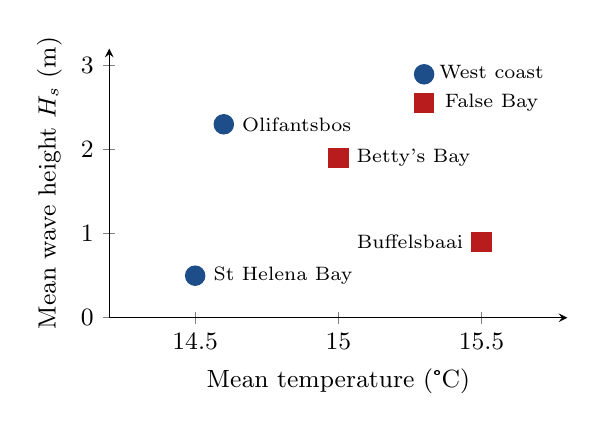
\begin{tikzpicture}
\begin{axis}[width=7.4cm, height=5.0cm, xmin=14.2, xmax=15.8, ymin=0, ymax=3.2,
  xlabel={\small Mean temperature (\textdegree C)}, ylabel={\small Mean wave height $H_s$ (m)},
  xticklabel style={font=\small, /pgf/number format/fixed, /pgf/number format/precision=1}, yticklabel style={font=\small}, axis lines=left, clip=false,
  legend style={font=\scriptsize, at={(0.98,0.98)}, anchor=north east, draw=none, fill=none}]
  \addplot[only marks, mark=*, mark size=3.5pt, sea] coordinates {(14.5,0.5) (14.6,2.3)};
  \addplot[only marks, mark=square*, mark size=3.5pt, hot] coordinates {(15.5,0.9) (15.0,1.9)};
  \legend{West coast, False Bay}
  \node[font=\scriptsize, anchor=west] at (axis cs:14.53,0.5) {St Helena Bay};
  \node[font=\scriptsize, anchor=west] at (axis cs:14.63,2.3) {Olifantsbos};
  \node[font=\scriptsize, anchor=east] at (axis cs:15.47,0.9) {Buffelsbaai};
  \node[font=\scriptsize, anchor=west] at (axis cs:15.03,1.9) {Betty's Bay};
\end{axis}
\end{tikzpicture}
\fignote{Annual means, end sites of each coast: Coppin et al.\ (2020).}}
\end{frame}

% 15 --------------------------------------------------------------------
\begin{frame}{Extremes are becoming more common}
\pb{climate change}
\twocol{
\begin{itemize}
  \item Marine heatwaves, 1925--2016 (global average):
  \begin{itemize}
    \item frequency +34\%; duration +17\%
    \item heatwave days per year +54\%
  \end{itemize}
  \item Most of the trend follows the rise in mean ocean temperature
  \item On land, hot and dry extremes increasingly occur together
\end{itemize}}{
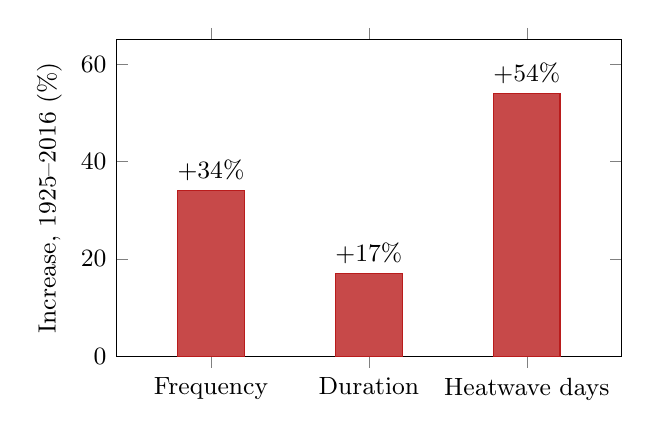
\begin{tikzpicture}
\begin{axis}[ybar, width=8.0cm, height=5.6cm, bar width=24pt, ymin=0, ymax=65,
  symbolic x coords={Frequency,Duration,Days}, xtick=data,
  xticklabels={Frequency, Duration, Heatwave days},
  xticklabel style={font=\small}, yticklabel style={font=\small},
  ylabel={\small Increase, 1925--2016 (\%)},
  nodes near coords, nodes near coords={+\pgfmathprintnumber{\pgfplotspointmeta}\%}, every node near coord/.append style={font=\small}, enlarge x limits=0.3]
\addplot[fill=hot!80, draw=hot] coordinates {(Frequency,34) (Duration,17) (Days,54)};
\end{axis}
\end{tikzpicture}
\fignote{Data: Oliver et al. (2018).}}
\end{frame}

% 16 --------------------------------------------------------------------
\begin{frame}{Stress and food: crop yields in a warmer world}
\pb{climate change, freshwater}
\twocol{
\begin{itemize}
  \item Four crops supply about two-thirds of human calories
  \item Each 1\,\textdegree C of global warming reduces average yields, if there is no CO$_2$ fertilisation, adaptation or breeding
  \item Effects vary strongly among regions
  \item Heat is more damaging when combined with drought
\end{itemize}}{
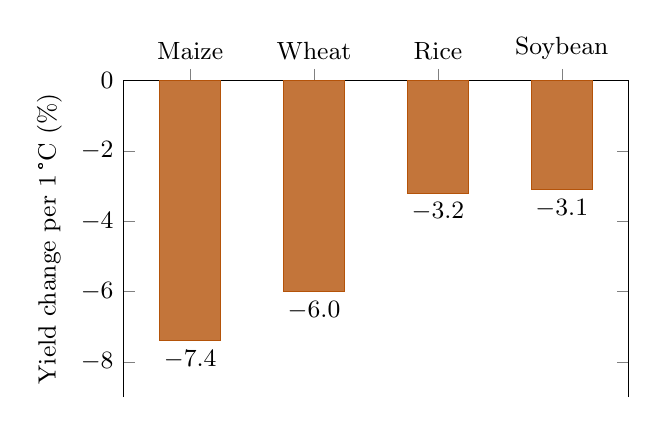
\begin{tikzpicture}
\begin{axis}[ybar, width=8.0cm, height=5.6cm, bar width=22pt, ymin=-9, ymax=0,
  symbolic x coords={Maize,Wheat,Rice,Soybean}, xtick=data, xticklabel pos=upper,
  xticklabel style={font=\small}, yticklabel style={font=\small},
  ylabel={\small Yield change per 1\,\textdegree C (\%)},
  nodes near coords, nodes near coords={\pgfmathprintnumber[fixed,precision=1,fixed zerofill]{\pgfplotspointmeta}}, every node near coord/.append style={font=\small, anchor=north}, enlarge x limits=0.18,
  axis x line*=top]
\addplot[fill=warm!80, draw=warm] coordinates {(Maize,-7.4) (Wheat,-6.0) (Rice,-3.2) (Soybean,-3.1)};
\end{axis}
\end{tikzpicture}
\fignote{Data: Zhao et al. (2017); heat--drought interaction: Matiu et al. (2017).}}
\end{frame}

% 17 --------------------------------------------------------------------
\begin{frame}{Stress and forests: hotter droughts}
\pb{climate change, freshwater, land system}
\twocol{
\begin{itemize}
  \item Drought- and heat-induced tree die-off reported on every forested continent
  \item A global database: 154 studies, 675 locations, 1303 plots
  \item Mortality years were hotter \textbf{and} drier than normal: a ``hotter-drought fingerprint''
  \item Lost trees mean lost carbon storage: a feedback to climate (Lecture 5)
\end{itemize}}{
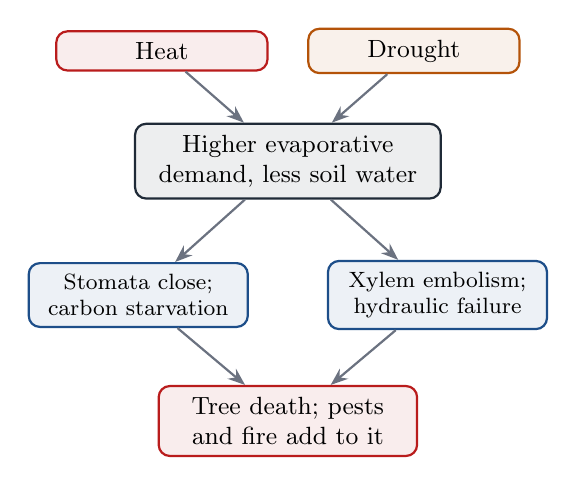
\begin{tikzpicture}[font=\small]
  \node[flow=hot, text width=2.4cm] (h) at (-1.6,2.2) {Heat};
  \node[flow=warm, text width=2.4cm] (d) at (1.6,2.2) {Drought};
  \node[flow=ink, text width=3.6cm] (v) at (0,0.8) {Higher evaporative demand, less soil water};
  \node[flow=sea, text width=2.5cm, font=\footnotesize] (x) at (-1.9,-0.9) {Stomata close; carbon starvation};
  \node[flow=sea, text width=2.5cm, font=\footnotesize] (e) at (1.9,-0.9) {Xylem embolism; hydraulic failure};
  \node[flow=hot, text width=3.0cm] (m) at (0,-2.5) {Tree death; pests and fire add to it};
  \draw[arr] (h) -- (v); \draw[arr] (d) -- (v); \draw[arr] (v) -- (x); \draw[arr] (v) -- (e); \draw[arr] (x) -- (m); \draw[arr] (e) -- (m);
\end{tikzpicture}
\fignote{Allen et al. (2010); Hammond et al. (2022).}}
\end{frame}

% 18 --------------------------------------------------------------------
\begin{frame}{Many small stresses add up}
\pb{several at once}
\twocol{
\begin{itemize}
  \item In nature, stresses rarely come one at a time
  \item \textit{Arabidopsis} seedlings were given up to six different stresses (including heat, salt, high light, a herbicide and cadmium), each at a mild level
  \item Each stress alone had little effect
  \item Together, growth and survival declined steeply as the number of stresses increased
\end{itemize}}{
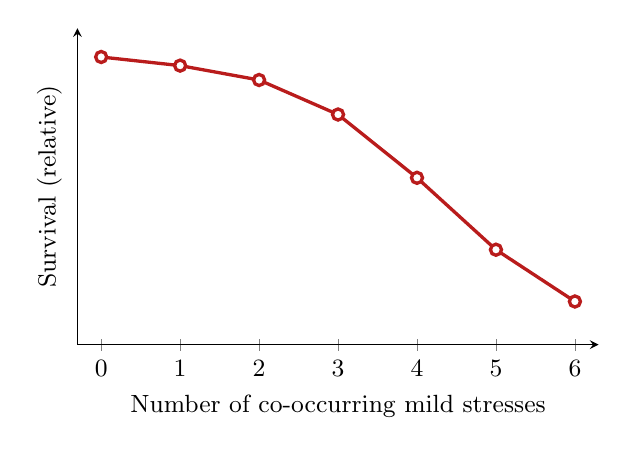
\begin{tikzpicture}
\begin{axis}[width=8.2cm, height=5.6cm, xmin=-0.3, xmax=6.3, ymin=0, ymax=1.1,
  axis lines=left, xtick={0,1,...,6}, ytick=\empty, xticklabel style={font=\small},
  xlabel={\small Number of co-occurring mild stresses}, ylabel={\small Survival (relative)}]
  \addplot[very thick, hot, mark=*, mark options={fill=white}] coordinates {(0,1) (1,0.97) (2,0.92) (3,0.80) (4,0.58) (5,0.33) (6,0.15)};
\end{axis}
\end{tikzpicture}
\fignote{Schematic of the trend reported by Zandalinas et al. (2021); not their data.}}
\end{frame}

% 19 --------------------------------------------------------------------
\begin{frame}{Summary}
\begin{itemize}
  \item Stress is any condition that limits metabolism, growth or development; it is defined relative to the plant
  \item Each plant has a tolerance curve; stress begins where function falls below the optimum
  \item Stress unfolds in phases: alarm, resistance, exhaustion or regeneration
  \item Many stresses converge on photosynthesis: absorbed energy exceeds what can be used, and ROS form
  \item Plants \textbf{avoid}, \textbf{tolerate} (by acclimation) or \textbf{succumb}
  \item Regulation (seconds), acclimation (days), morphological plasticity (months) and adaptation (generations)
  \item Each crossed planetary boundary is a stressor; together they add extremes and combine stresses
\end{itemize}
\end{frame}

\end{document}
